\documentclass[12pt]{scrartcl}

\usepackage{amsmath,amssymb}
\usepackage{fullpage}
\usepackage{hyperref}
\usepackage{graphicx}
\usepackage{tikz}
\usepackage[inline]{enumitem}
\usepackage{tabularx}
\usepackage{array}

\newcolumntype{Y}{>{\centering\arraybackslash}X}
\newcolumntype{L}[1]{>{\raggedright\arraybackslash}p{#1}}
\newcolumntype{C}[1]{>{\centering\arraybackslash}p{#1}}

\setlist[enumerate,1]{label=\alph*), itemjoin=\hspace{1.2em}, itemjoin*=\hspace{1.2em}}

\usetikzlibrary{calc}

\setlength{\parindent}{0pt}

\begin{document}

\begin{center}
	\hrule
	\vspace{0.4cm}
	{\textbf{\large Tutorial 01}}\\ [0.2cm]
	INF1004 Mathematics II

\end{center}

\textbf{Name:} Timothy Chia \hspace{\fill} \textbf{Date:} - \\

\hrule

\begin{enumerate}[label=\textbf{\arabic*.}]

	\item  In a sample of 20 people the times taken, in seconds, to solve a simple numerical puzzle
	      were as follows:

	      \begin{center}
		      \begin{tabular}{c c c c c c c c c c}
			      17 & 19 & 22 & 26 & 28 & 31 & 34 & 36 & 38 & 39 \\
			      41 & 42 & 43 & 47 & 50 & 51 & 53 & 55 & 57 & 58 \\
		      \end{tabular}
	      \end{center}

	      \begin{enumerate}[label=(\alph*)]
		      \item Calculate the mean and standard deviation of these times.
		      \item In fact, 23 people attempted to solve this puzzle. However, 3 of them failed to solve it within the allotted time of 60 seconds, taking 62, 65 and 97 seconds respectively.\\[0.5cm] Calculate the interquartile range (IQR) of the times taken by all 23 people.
		      \item Are there any outliers in the dataset?
	      \end{enumerate}

	      \medskip

	      \textbf{Solution.}
	      %------------------------------------------------------------

	      \begin{enumerate}[label=(\alph*)]
		      \item The sample mean is
		            \[
			            \bar{x}=\frac{\sum_{i=1}^{20} x_i}{20}
			            =\frac{787}{20}=39.35\text{ s}.
		            \]
		            The sample variance is
		            \[
			            s^2=\frac{1}{n-1}\sum_{i=1}^{n}(x_i-\bar{x})^2
			            =\frac{3054.55}{19}=160.7658.
		            \]
		            Hence the sample standard deviation is
		            \[
			            s=\sqrt{s^2}=\sqrt{160.7658}=12.679\text{ s}\quad (\text{3 d.p.}).
		            \]

		      \item Including the additional three times, the ordered data set is
		            \[
			            17,\,19,\,22,\,26,\,28,\,31,\,34,\,36,\,38,\,39,\,41,\,42,\,43,\,47,\,50,\,51,\,53,\,55,\,57,\,58,\,62,\,65,\,97.
		            \]
		            With $n=23$, the median is the $12$th value, so $Q_2=42$.
		            The lower half has $11$ values, so $Q_1$ is its median: $Q_1=31$.
		            The upper half has $11$ values, so $Q_3$ is its median: $Q_3=55$.
		            Therefore,
		            \[
			            \mathrm{IQR}=Q_3-Q_1=55-31=24.
		            \]

		      \item The outlier fences are
		            \[
			            \text{Lower fence}=Q_1-1.5(\mathrm{IQR})=31-1.5(24)=-5,
		            \]
		            \[
			            \text{Upper fence}=Q_3+1.5(\mathrm{IQR})=55+1.5(24)=91.
		            \]
		            Since $97>91$, the value $97$ is an outlier.
	      \end{enumerate}


	      % -----------------------------------------------------------


	      \newpage
	\item Consider the following tree diagram. \\ [0.2cm]

	      \noindent\makebox[\textwidth][c]{%  
		      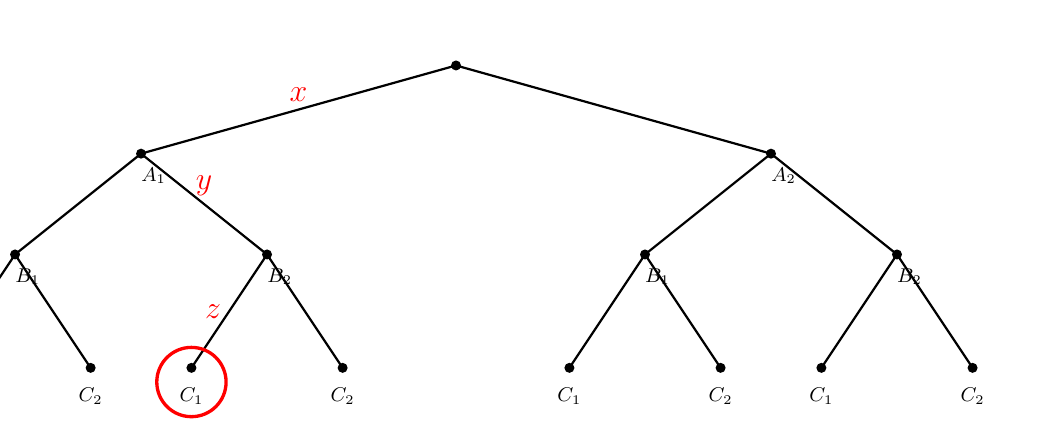
\begin{tikzpicture}[line cap=round, line join=round, thick, scale=0.80, transform shape]
			      \useasboundingbox (-6.8,-5.6) rectangle (9,0.6);
			      \tikzset{
				      dot/.style={circle, fill=black, inner sep=1.6pt},
				      lab/.style={font=\small},
				      redlab/.style={red, font=\Large\bfseries\itshape}
			      }

			      % --- coordinates (tweak if you want different spacing)
			      \coordinate (R)  at (0,0);

			      \coordinate (A1) at (-5,-1.4);
			      \coordinate (A2) at ( 5,-1.4);

			      \coordinate (B11) at (-7,-3.0);
			      \coordinate (B12) at (-3,-3.0);

			      \coordinate (C111) at (-8.2,-4.8);
			      \coordinate (C112) at (-5.8,-4.8);

			      \coordinate (C121) at (-4.2,-4.8); % this is the circled C1
			      \coordinate (C122) at (-1.8,-4.8);

			      \coordinate (B21) at ( 3,-3.0);
			      \coordinate (B22) at ( 7,-3.0);

			      \coordinate (C211) at ( 1.8,-4.8);
			      \coordinate (C212) at ( 4.2,-4.8);

			      \coordinate (C221) at ( 5.8,-4.8);
			      \coordinate (C222) at ( 8.2,-4.8);

			      % --- edges + red edge labels
			      \draw (R) -- (A1) node[midway, above, redlab] {$x$};
			      \draw (R) -- (A2);

			      \draw (A1) -- (B11);
			      \draw (A1) -- (B12) node[midway, above, redlab] {$y$};

			      \draw (B11) -- (C111);
			      \draw (B11) -- (C112);

			      \draw (B12) -- (C121) node[midway, left, redlab] {$z$};
			      \draw (B12) -- (C122);

			      \draw (A2) -- (B21);
			      \draw (A2) -- (B22);

			      \draw (B21) -- (C211);
			      \draw (B21) -- (C212);

			      \draw (B22) -- (C221);
			      \draw (B22) -- (C222);

			      % --- dots at all nodes
			      \node[dot] at (R)   {};
			      \node[dot] at (A1)  {};
			      \node[dot] at (A2)  {};

			      \node[dot] at (B11) {};
			      \node[dot] at (B12) {};
			      \node[dot] at (B21) {};
			      \node[dot] at (B22) {};

			      \node[dot] at (C111) {};
			      \node[dot] at (C112) {};
			      \node[dot] at (C121) {};
			      \node[dot] at (C122) {};

			      \node[dot] at (C211) {};
			      \node[dot] at (C212) {};
			      \node[dot] at (C221) {};
			      \node[dot] at (C222) {};

			      % --- labels near nodes (slightly offset to mimic the figure)
			      \node[lab] at ($(A1)+(0.20,-0.35)$) {$A_1$};
			      \node[lab] at ($(A2)+(0.20,-0.35)$) {$A_2$};

			      \node[lab] at ($(B11)+(0.20,-0.35)$) {$B_1$};
			      \node[lab] at ($(B12)+(0.20,-0.35)$) {$B_2$};
			      \node[lab] at ($(B21)+(0.20,-0.35)$) {$B_1$};
			      \node[lab] at ($(B22)+(0.20,-0.35)$) {$B_2$};

			      \node[lab] (c111lab) at ($(C111)+(0.00,-0.45)$) {$C_1$};
			      \node[lab] (c112lab) at ($(C112)+(0.00,-0.45)$) {$C_2$};

			      \node[lab] (c121lab) at ($(C121)+(0.00,-0.45)$) {$C_1$};
			      \node[lab] (c122lab) at ($(C122)+(0.00,-0.45)$) {$C_2$};

			      \node[lab] (c211lab) at ($(C211)+(0.00,-0.45)$) {$C_1$};
			      \node[lab] (c212lab) at ($(C212)+(0.00,-0.45)$) {$C_2$};

			      \node[lab] (c221lab) at ($(C221)+(0.00,-0.45)$) {$C_1$};
			      \node[lab] (c222lab) at ($(C222)+(0.00,-0.45)$) {$C_2$};

			      % --- red circle around the left-subtree C1 under B2
			      \draw[red, very thick]
			      ($(C121)!0.5!(c121lab)$) circle [radius=0.55];

		      \end{tikzpicture}
	      }

	      \begin{enumerate}[label=(\alph*)]
		      \item What does the probability $x$ represent?

		            \begin{enumerate*}[label=\alph*)]
			            \item $P(A_1)$ \quad \quad
			            \item $P(A_1 \mid B_2)$ \quad \quad
			            \item $P(B_2 \mid A_1)$ \quad \quad
			            \item $P(C_1 \mid B_2 \cap A_1)$ \quad \quad
		            \end{enumerate*}

		            \medskip

		      \item What does the probability $y$ represent?

		            \begin{enumerate*}[label=\alph*)]
			            \item $P(B_2)$ \quad \quad
			            \item $P(A_1\mid B_2)$ \quad \quad
			            \item $P(B_2\mid A_1)$ \quad \quad
			            \item $P(C_1\mid B_2 \cap A_1)$ \quad \quad
		            \end{enumerate*}

		            \medskip

		      \item The probability $z$ represents?

		            \begin{enumerate*}[label=\alph*)]
			            \item $P(C_1)$ \quad \quad
			            \item $P(B_2\mid C_1)$ \quad \quad
			            \item $P(C_1\mid B_2)$ \quad \quad
			            \item $P(C_1\mid B_2 \cap A_1)$ \quad \quad
		            \end{enumerate*}

		            \medskip

		      \item The circled node represents the event?

		            \begin{enumerate*}[label=\alph*)]
			            \item $C_1$ \quad \quad
			            \item $B_2 \cap C_1$ \quad \quad
			            \item $A_1 \cap B_2 \cap C_1$ \quad \quad
			            \item $C_1 \mid (B_2 \cap A_2)$ \quad \quad
		            \end{enumerate*}

		            \medskip

		      \item Let $A$ and $B$ be two events. Suppose that the probability that neither event occurs is $\tfrac{3}{8}$.
		            What is the probability that at least one of the events occurs?

		            \medskip

		      \item Let $C$ and $D$ be two events. Suppose $P(C)=0.5$, $P(C\cap D)=0.2$ and $P\big((C\cup D)^c\big)=0.4$.
		            What is $P(D)$?
	      \end{enumerate}

	      \medskip

	      \textbf{Solution.}

	      \begin{enumerate}[label=(\alph*)]
		      \item Since $x$ labels the branch from the root to $A_1$, we have $x=P(A_1)$.

		      \item Since $y$ labels the branch from $A_1$ to $B_2$, we have $y=P(B_2\mid A_1)$.

		      \item Since $z$ labels the branch from $A_1\cap B_2$ to $C_1$, we have $z=P(C_1\mid A_1\cap B_2)$.

		      \item The circled node corresponds to the event $A_1\cap B_2\cap C_1$.

		      \item If $P(A^c\cap B^c)=\tfrac{3}{8}$, then by De Morgan's law,
		            \[
			            P(A\cup B)=1-P\big((A\cup B)^c\big)=1-P(A^c\cap B^c)=1-\frac{3}{8}=\frac{5}{8}.
		            \]

		      \item We are given $P(C)=0.5$, $P(C\cap D)=0.2$ and $P\big((C\cup D)^c\big)=0.4$.
		            Then $P(C\cup D)=1-0.4=0.6$, and by inclusion--exclusion,
		            \[
			            P(C\cup D)=P(C)+P(D)-P(C\cap D).
		            \]
		            Hence
		            \[
			            0.6=0.5+P(D)-0.2 \quad\Rightarrow\quad P(D)=0.3.
		            \]
	      \end{enumerate}

	\item In a survey of 1929 students, the following data were obtained on ``students' first reason
	      for application to the university in which they matriculated.''

	      \medskip

	      \begin{center}
		      \small
		      \setlength{\tabcolsep}{6pt}
		      \renewcommand{\arraystretch}{1.2}

		      \begin{tabular}{p{0.25\linewidth}|c c c|c}
			      \textbf{Enrollment status} &
			      \textbf{\shortstack{University                      \\Quality}} &
			      \textbf{\shortstack{University Cost                 \\or Convenience}} &
			      \textbf{Other}             &
			      \textbf{Total}                                      \\
			      \hline
			      Full-time                  & 421 & 393 & 76  & 890  \\
			      Part-time                  & 400 & 593 & 46  & 1039 \\
			      \hline
			      Total                      & 821 & 986 & 122 & 1929 \\
		      \end{tabular}
	      \end{center}

	      \medskip

	      \begin{enumerate}[label=(\alph*)]
		      \item What is the probability that university quality is the first reason for a student to choose a university?
		      \item For a full-time student, what is the probability that university quality is the first reason for choosing a university?
		      \item Let $A$ denote the event that a student is full-time, and let $B$ denote the event that the student
		            lists university quality as the first reason for applying. Are events $A$ and $B$ independent?
	      \end{enumerate}

	      \medskip

	      \textbf{Solution.}
	      \begin{enumerate}[label=(\alph*)]
		      \item $P(A)=\frac{821}{1929}\approx 0.4256$.

		      \item $P(B\mid A)=\frac{421}{890}\approx 0.4730$.

		      \item
		            To test independence, we can check whether $P(B\mid A)=P(B)$ (equivalently, whether
		            $P(A\cap B)=P(A)P(B)$).

		            From the given fractions,
		            \[
			            P(B)=\frac{821}{1929}\approx 0.4256,
			            \qquad
			            P(B\mid A)=\frac{421}{890}\approx 0.4730.
		            \]
		            Since
		            \[
			            P(B\mid A)\neq P(B)
			            \quad\text{(i.e. }0.4730\neq 0.4256\text{),}
		            \]
		            events $A$ and $B$ are \textbf{not independent}.

		            We can also verify this using $P(A\cap B)=P(A)P(B)$:
		            \[
			            P(A)=\frac{890}{1929}\approx 0.4614,
			            \qquad
			            P(A\cap B)=\frac{421}{1929}\approx 0.2183.
		            \]
		            But
		            \[
			            P(A)P(B)=\left(\frac{890}{1929}\right)\left(\frac{821}{1929}\right)
			            \approx 0.1965 \neq 0.2183 \approx P(A\cap B).
		            \]
		            Therefore, events $A$ and $B$ are \textbf{dependent}.


	      \end{enumerate}

	      %------------------------------------------------------------
	      \newpage
	\item A rare blood disease is found in 2\% of a certain population. A new blood test can correctly
	      identify 96\% of the people with the disease and 94\% of the people without the disease.

	      \begin{enumerate}[label=(\alph*)]
		      \item What is the probability that a person who is tested positive by the blood test actually has the disease?
		      \item What is the probability that a person who is tested negative by the blood test actually does not have the disease?
	      \end{enumerate}

	      \medskip

	      \textbf{Solution.}
	      \begin{enumerate}[label=(\alph*)]
		      \item
		            Let $A$ be the event that a person has the disease, and $B$ be the event that the person tests positive.
		            We are given
		            \[
			            P(A)=0.02,\quad P(A^c)=0.98,\quad P(B\mid A)=0.96,\quad P(B^c\mid A^c)=0.94.
		            \]
		            First find the false positive rate:
		            \[
			            P(B\mid A^c)=1-P(B^c\mid A^c)=1-0.94=0.06.
		            \]
		            Using Bayes' theorem,
		            \[
			            P(A\mid B)=\frac{P(B\mid A)P(A)}{P(B\mid A)P(A)+P(B\mid A^c)P(A^c)}
			            =\frac{0.96(0.02)}{0.96(0.02)+0.06(0.98)}.
		            \]
		            Therefore,
		            \[
			            P(A\mid B)=\frac{0.0192}{0.0192+0.0588}
			            =\frac{0.0192}{0.078}
			            \approx 0.2462.
		            \]

		      \item
		            We want the probability that a person who tests negative does \emph{not} have the disease, i.e.
		            \[
			            P(A^c\mid B^c).
		            \]
		            First find the false negative rate:
		            \[
			            P(B^c\mid A)=1-P(B\mid A)=1-0.96=0.04.
		            \]
		            Then
		            \[
			            P(A^c\cap B^c)=P(B^c\mid A^c)P(A^c)=0.94(0.98)=0.9212,
		            \]
		            \[
			            P(A\cap B^c)=P(B^c\mid A)P(A)=0.04(0.02)=0.0008,
		            \]
		            so
		            \[
			            P(B^c)=P(A^c\cap B^c)+P(A\cap B^c)=0.9212+0.0008=0.922.
		            \]
		            Hence,
		            \[
			            P(A^c\mid B^c)=\frac{P(A^c\cap B^c)}{P(B^c)}
			            =\frac{0.9212}{0.922}
			            \approx 0.9991.
		            \]
	      \end{enumerate}

	      %------------------------------------------------------------
	      \newpage
	\item A woman is pregnant with male twins. Twins may be either identical or fraternal (non-identical).
	      In general, $\tfrac{1}{3}$ twins born are identical. Obviously, identical twins must be of the same sex;
	      fraternal twins may or may not be. Assume that identical twins are equally likely to be both boys or both girls,
	      while for fraternal twins all possibilities are equally likely: boy-girl, girl-boy, boy-boy, girl-girl.
	      Given the above information, what is the probability that the woman's male twins are identical?

	      \medskip
	      \textbf{Solution.}

	      Let $I$ be the event that a woman is pregnant with \textbf{identical} twins, and let $F$ be the event that she is pregnant with \textbf{fraternal} twins. We are given
	      \[
		      P(I)=\frac13
		      \qquad\Rightarrow\qquad
		      P(F)=1-P(I)=\frac23.
	      \]
	      Let $B$ be the event that \textbf{both twins are boys}. We want to find $P(I\mid B)$.

	      If the twins are identical, they must be the same sex (either $BB$ or $GG$), and these two outcomes are equally likely, so
	      \[
		      P(B\mid I)=\frac12.
	      \]
	      If the twins are fraternal, the four outcomes $BB, BG, GB, GG$ are equally likely, hence
	      \[
		      P(B\mid F)=\frac14.
	      \]

	      Using Bayes' Theorem,
	      \[
		      P(I\mid B)=\frac{P(B\mid I)\,P(I)}{P(B\mid I)\,P(I)+P(B\mid F)\,P(F)}.
	      \]
	      Substituting values gives
	      \[
		      P(I\mid B)=\frac{\left(\frac12\right)\left(\frac13\right)}
		      {\left(\frac12\right)\left(\frac13\right)+\left(\frac14\right)\left(\frac23\right)}
		      =\frac{\frac16}{\frac16+\frac16}
		      =\frac12.
	      \]

	      \[
		      P(I\mid B)=\frac12.
	      \]

	      %------------------------------------------------------------
	      \newpage
	\item If a family had three kids, named Alice, Bob, and Carl. Assume that each is equally likely to be born;
	      i.e., $1/3$ chance for each of them to be born first etc.

	      \begin{enumerate}[label=(\alph*)]
		      \item Find the probability that Alice is older than Bob, given that Alice is older than Carl.
		      \item Is event ``Alice is older than Bob'' independent from event ``Alice is older than C''?
	      \end{enumerate}

	      \medskip

	      \textbf{Solution.}

	      Let $S$ be the sample space containing all possible birth sequences:
	      \[
		      S=\{ABC,\,ACB,\,BAC,\,BCA,\,CAB,\,CBA\}.
	      \]

	      \begin{itemize}
		      \item[(a)] Let $A$ be the event that Alice is born before Carl. Then
		            \[
			            A=\{ABC,\,ACB,\,BAC\}
			            \qquad\Rightarrow\qquad
			            P(A)=\frac{3}{6}=\frac12.
		            \]
		            Let $B$ be the event that Alice is born before Bob, given that Alice is born before Carl.
		            Within $A$, the outcomes are $ABC, ACB, BAC$, and Alice is born before Bob in $ABC$ and $ACB$, so
		            \[
			            P(B\mid A)=\frac{2}{3}.
		            \]

		      \item[(b)] Using the same events
		            \[
			            A=\{\text{Alice is born before Carl}\},
			            \qquad
			            B=\{\text{Alice is born before Bob}\},
		            \]
		            we have
		            \[
			            P(A)=\frac12,
			            \qquad
			            P(B)=\frac12.
		            \]
		            Also,
		            \[
			            A\cap B=\{ABC,\,ACB\}
			            \qquad\Rightarrow\qquad
			            P(A\cap B)=\frac{2}{6}=\frac13.
		            \]
		            Since
		            \[
			            P(A\cap B)=\frac13 \neq \frac12\cdot\frac12=\frac14,
		            \]
		            the events $A$ and $B$ are \textbf{not independent}.
	      \end{itemize}

	      %------------------------------------------------------------
	      \newpage
	\item A boy receives a school report card each week. He is given a special treat whenever his report indicates
	      ``Good behavior'' \textbf{AND} ``Excellent Homework''. His behavior is good with probability 0.6.
	      When his behavior is good, he has a probability of 0.8 of doing excellent homework. When his behavior is not good,
	      his probability of doing excellent homework is only 0.5.

	      \begin{enumerate}[label=(\alph*)]
		      \item For a random week, calculate the probability that he will be given a special treat.
		      \item For a random week, calculate the probability that his homework will be excellent but he will not be given a special treat.
		      \item For a random week, calculate the probability that his homework will be excellent.
		      \item Given that his homework is excellent, calculate the conditional probability that he is \textbf{NOT} given a special treat.
	      \end{enumerate}

	      \medskip

	      \textbf{Solution.}


	      Let $G$ be the event of \textbf{good behaviour} and let $E$ be the event of \textbf{excellent homework}.
	      We are given
	      \[
		      P(G)=0.6,\quad P(G^{c})=0.4,\quad P(E\mid G)=0.8,\quad P(E\mid G^{c})=0.5.
	      \]

	      \begin{itemize}
		      \item[(a)]
		            \[
			            P(G\cap E)=P(G)\,P(E\mid G)=(0.6)(0.8)=0.48.
		            \]

		      \item[(b)]
		            \[
			            P(G^{c}\cap E)=P(G^{c})\,P(E\mid G^{c})=(0.4)(0.5)=0.20.
		            \]

		      \item[(c)] Using that $E=(E\cap G)\cup(E\cap G^{c})$ with disjoint parts,
		            \[
			            P(E)=P(E\cap G)+P(E\cap G^{c})=0.48+0.20=0.68.
		            \]

		      \item[(d)] Let $N$ be the event of \textbf{no special treatment}.
		            A student gets special treatment iff $G\cap E$, so
		            \[
			            N=(G\cap E)^{c}=G^{c}\cup E^{c}.
		            \]
		            Given $E$ occurred,
		            \[
			            N\cap E = (G^{c}\cup E^{c})\cap E
			            =(G^{c}\cap E)\cup(E^{c}\cap E)
			            =G^{c}\cap E.
		            \]
		            Hence,
		            \[
			            P(N\mid E)=\frac{P(N\cap E)}{P(E)}
			            =\frac{P(G^{c}\cap E)}{P(E)}
			            =\frac{0.20}{0.68}
			            \approx 0.2941.
		            \]
	      \end{itemize}

	      %------------------------------------------------------------
	      \newpage
	\item In an attempt to find the mean number of hours his tutorial classmates spent per day preparing for tutorials,
	      John collected data from 10 of his friends in the tutorial group and found that the sample mean is 2.4 hours with a
	      sample standard deviation of 0.8 hours. However, a day later he felt that the sample size is too small.
	      So he collected data from another 5 of his friends and found that the sample mean is 2.0 hours with a sample
	      standard deviation of 1.2 hours.

	      \medskip

	      Find the sample mean and sample standard deviation \underline{when these 2 sets of data are combined}.

	      \medskip
	      \textbf{Solution.}

	      Group A (10 friends) has
	      \[
		      n_1=10,\qquad \bar{x}_1=2.4\text{ hours},\qquad s_1=0.8\text{ hours}.
	      \]
	      Group B (5 friends) has
	      \[
		      n_2=5,\qquad \bar{x}_2=2.0\text{ hours},\qquad s_2=1.2\text{ hours}.
	      \]
	      Let the combined group have size $n=n_1+n_2=15$.

	      \begin{itemize}
		      \item The combined mean is
		            \[
			            \bar{x}=\frac{n_1\bar{x}_1+n_2\bar{x}_2}{n_1+n_2}
			            =\frac{10(2.4)+5(2.0)}{15}
			            =\frac{34}{15}
			            \approx 2.27\text{ hours}.
		            \]

		      \item To find the combined standard deviation, combine sums of squares.
		            The within-group sums of squares are
		            \[
			            SS_1=(n_1-1)s_1^2=9(0.8^2)=5.76,
			            \qquad
			            SS_2=(n_2-1)s_2^2=4(1.2^2)=5.76.
		            \]
		            The between-group sum of squares is
		            \[
			            SS_{\text{between}}=n_1(\bar{x}_1-\bar{x})^2+n_2(\bar{x}_2-\bar{x})^2.
		            \]
		            Using $\bar{x}=\frac{34}{15}$,
		            \[
			            \bar{x}_1-\bar{x}=2.4-\frac{34}{15}=\frac{2}{15},
			            \qquad
			            \bar{x}_2-\bar{x}=2.0-\frac{34}{15}=-\frac{4}{15},
		            \]
		            so
		            \[
			            SS_{\text{between}}=10\left(\frac{2}{15}\right)^2+5\left(\frac{4}{15}\right)^2
			            =\frac{8}{15}\approx 0.5333.
		            \]
		            Hence the total sum of squares is
		            \[
			            SS=SS_1+SS_2+SS_{\text{between}}
			            =5.76+5.76+\frac{8}{15}
			            \approx 12.0533.
		            \]
		            The combined sample variance is
		            \[
			            s^2=\frac{SS}{n-1}=\frac{12.0533}{14}\approx 0.8610,
		            \]
		            so the combined sample standard deviation is
		            \[
			            s=\sqrt{0.8610}\approx 0.9279\text{ hours}.
		            \]
	      \end{itemize}

	      %------------------------------------------------------------
	      \newpage
	\item A certain family has 6 children, consisting of 3 boys and 3 girls. Assuming that all birth orders are equally likely,
	      what is the probability that the 3 eldest children are the 3 girls?

	      \medskip
	      \textbf{Solution.}

	      There are $6! = 720$ possible birth orders of the 6 children, and each order is equally likely.

	      To have the three girls in the first three positions, the girls can be arranged in $3!$ ways.
	      To have the three boys in the last three positions, the boys can be arranged in $3!$ ways.
	      Hence the number of favourable birth orders is
	      \[
		      3!\cdot 3! = 36,
	      \]
	      so
	      \[
		      P(\text{first three are girls and last three are boys})
		      =\frac{36}{720}
		      =\frac{1}{20}.
	      \]

	      Equivalently,
	      \[
		      P(\text{GGG then BBB})
		      =\frac{3}{6}\cdot\frac{2}{5}\cdot\frac{1}{4}
		      =\frac{1}{20}.
	      \]

\end{enumerate}

\end{document}
